% Metódy inžinierskej práce

\documentclass[12pt,a4paper]{article}
\usepackage[numbers]{natbib}
\usepackage{url}
\usepackage{tocloft}
\usepackage{xcolor}
\usepackage{titlesec}
\usepackage[hidelinks]{hyperref}
\usepackage{pgfplots}
\usepackage{pgf-pie}
\pgfplotsset{compat=1.18}





% Добавление точек от заголовка к номеру страницы
\renewcommand{\cftsecleader}{\cftdotfill{\cftdotsep}}
\renewcommand{\cftsubsecleader}{\cftdotfill{\cftdotsep}}


\title{How Streaming Services Use AI and Algorithms to Personalize Your Music Experience}
\author{Mykyta Nosenko}
\begin{document}
\maketitle
\section*{Abstarct}

Imagine you’re walking through a park, and everywhere you look, people are wearing headphones. Everyday, you can see hundreds or even thousands of individuals rapt in their own worlds of sound. What are they listening to? Some may be tuned into podcasts, audiobooks, or radio, but most are likely enjoying music. In today’s digital age, powerful streaming services like Spotify make accessing our favorite songs effortless. In this article, we will dive into how their recommendation systems work.

We’re about to explore the enormous world of algorithms and artificial intelligence that recommend songs specifically tailored to our tastes. At the heart of Spotify’s recommendation engine are algorithms like collaborative filtering and content-based filtering. For example, collaborative filtering uses matrix factorization to identify hidden user preferences based on listening habits, while content-based filtering employs techniques like TF-IDF to analyze song lyrics and extract significant themes. Additionally, Spotify leverages an AI system called Marlin, which combines these algorithms to enhance user experience and provide personalized music recommendations\citep{href}.

How do these systems understand our preferences? Who develops these complex technologies, and what exactly goes into building them? There are so many questions, and much remains unknown about how AI enhances our music experience, constantly adapting to our moods and listening habits. Let's take a closer look at how it all works.

\newpage
\tableofcontents
\newpage

\section{Recommendation Systems An Overview}



Greetings to everyone! I hope your mood is great and everything is going according to plan. Before we begin, try to clear your mind of distractions and fully immerse yourself in the topic. How do development teams within giants like Spotify, Yandex Music, Apple Music, and Deezer work — from solving complex tasks to team-building activities? Is machine learning involved? On what basis are recommendations made, and how do music services select the perfect playlists for us? So many questions, and there's so much to discover in this article. Let's dive in!

Modern music streaming services offer users not only access to extensive music catalogs but also ready-made playlists with personalized recommendations. Thanks to systems based on artificial intelligence and machine learning, the aforementioned platforms provide tracks that perfectly match each user's preferences. These systems play a crucial role in discovering new music. According to data from 2020, around 62\% of users identified Spotify and YouTube as the main sources for finding new tracks and artists.\citep{href}.

Today, we will explore how recommendation systems work on the biggest music platforms — Yandex Music, Spotify, Apple Music, and Deezer. Each of them is unique and holds a leading position on its continent.

\begin{itemize}
 \item \textbf{Yandex Music} — the leading music service in Russia and the CIS countries, offers access to a vast collection of tracks and uses sophisticated algorithms to analyze your musical preferences and moods.

\item \textbf{Spotify}, a Swedish platform popular in Europe and America, is renowned for its smart playlists and recommendations based on your tastes, time of day, and even your mood.

\item \textbf{Apple Music} — a global giant, popular in the USA and many other countries, is tightly integrated into the Apple ecosystem. It uses your listening habits and interactions with music to create a personalized experience.

\item \textbf{Deezer}, a French leader, has gained popularity in Europe thanks to localized recommendations and unique algorithms that adapt music selections to each user as much as possible.
\end{itemize}

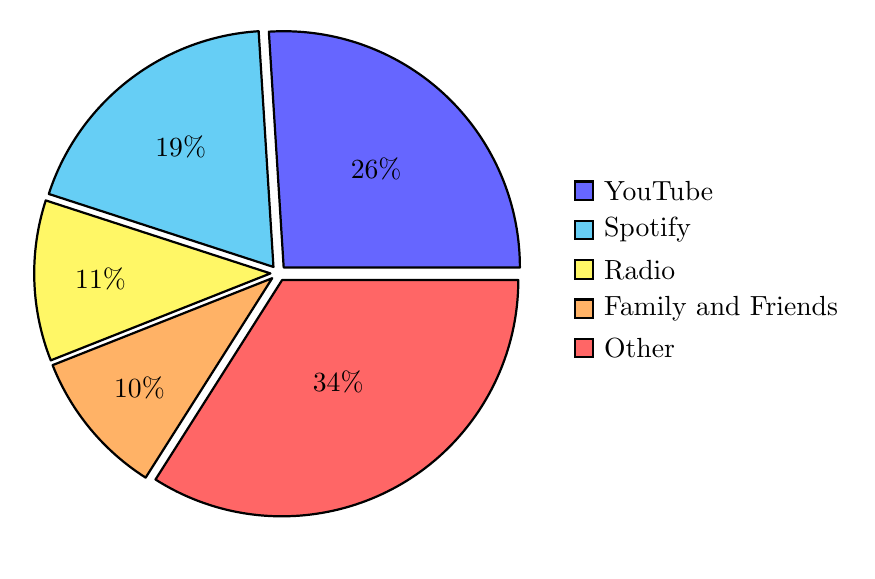
\begin{tikzpicture}
    \pie[
        text=legend, 
        radius=3, 
        explode=0.1 
    ]{
        26/YouTube,
        19/Spotify,
        11/Radio,
        10/Family and Friends,
        34/Other
    }
\end{tikzpicture}

We have gathered information from podcasts and interviews with company executives and developers to better understand how these systems are built and what technologies power them. Ready to embark on a journey into the world of music technology? Let's go!

\section{Algorithms Behind the Recommendation System of Yandex Music}

\section{The Role of Artificial Intelligence}

\section{The Future of Recommendation Systems}

\section{Conclusion}

\newpage
\section{References}

\bibliographystyle{abbrvnat}
\bibliography{MainBIB.bib}

\end{document}











